% Сглаживание границ доменов.
\subsection{Сглаживание границ между доменами поверхностной расчетной сетки}

\subsubsection{Алгоритм сглаживания границ между доменами}

Алгоритм сглаживания носит локальный характер, он применяется последовательно к каждой паре доменов и направлен на уменьшение длины границы между ними с сохранением баланса количества ячеек в этих доменах.
Граница между двумя доменами может быть представлена в виде набора простых циклов и простых цепей.
При этом простой цикл может быть обработан таким же образом, как и простая цепь, с учетом совпадения первого и последнего узла этой цепи (для такого виртуального размыкания простого цикла может быть выбран произвольный узел этого цикла).
В процессе применения алгоритма сглаживания независимо обрабатывается каждая цепь.

Вначале одним линейным проходом по цепи выполняется поиск всех пригодных для оптимизации границы шаблонов, представленных на рис.~\ref{fig:text_2_smooth_smooth_border}.

\begin{figure}[ht]
	\centering
	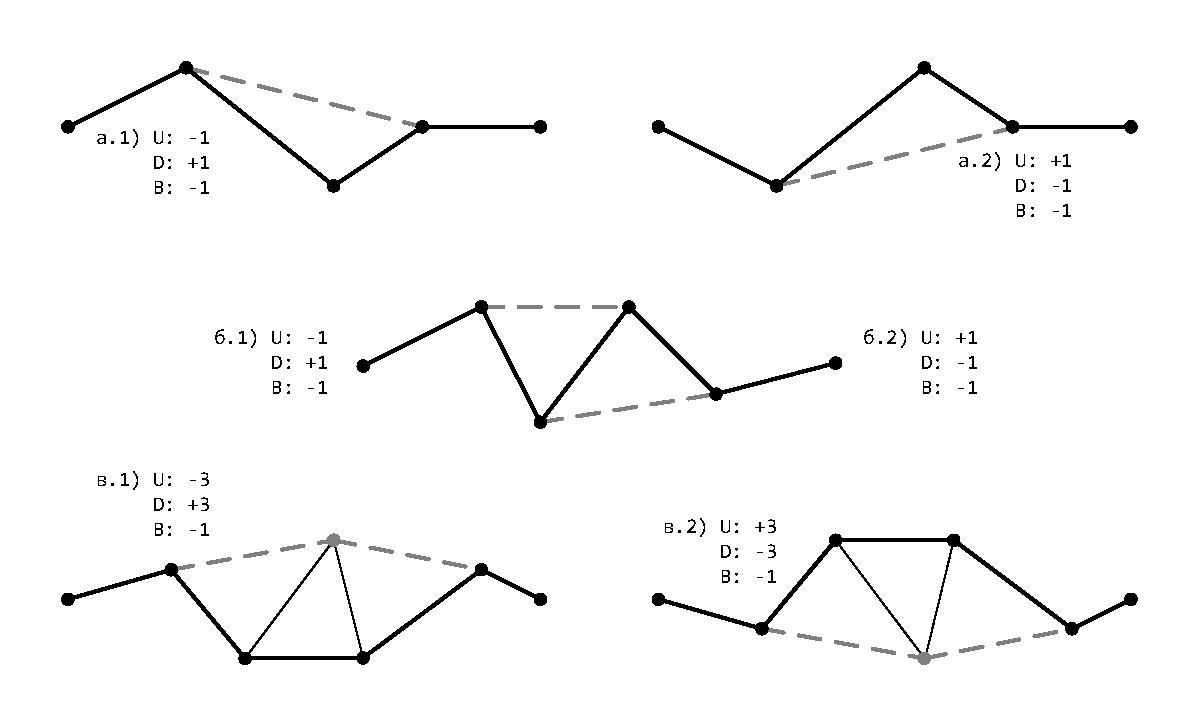
\includegraphics[width=0.8\textwidth]{./pics/text_2_smooth/smooth-border.pdf}
	\caption{Шаблоны элементарных действий сглаживания границ между доменами.}
	\label{fig:text_2_smooth_smooth_border}
\end{figure}

На рис.~\ref{fig:text_2_smooth_smooth_border} представлены 5 шаблонов, которые могут быть использованы для оптимизации длины границы между двумя доменами.
Рассмотрим шаблон а.1.
На нем обозначена часть границы между двумя доменами (домен сверху от ломаной обозначен буквой $U$, домен снизу от ломаной обозначен буквой $D$.
Черной сплошной линией прочерчена текущая граница между доменами.
Пунктирной линией показано возможное улучшение, которое в данном случае приведет к следующим последствиям: уменьшение количества ячеек верхнего домена на 1 ($U: -1$), увеличение количества ячеек нижнего домена на 1 ($D: + 1$), уменьшение длины границы между двумя доменами на 1 ($B: -1$).
Таким образом, шаблон а.1 направлен на втягивание одной ячейки из верхнего домена в нижний домен с сокращением длины границы на единицу.
Шаблон а.2 выполняет симметричное действие по втягиванию одной ячейки из нижнего домена в верхний домен, также сокращая при этом длину границы на единицу.
Шаблоны в.1 и в.2 выполняют аналогичные действия, однако вместо одной ячейки происходит втягивание сразу трех соседних ячеек с одновременным уменьшением длины границы между доменами на единицу. Отдельно стоит отметить шаблоны б.1 и б.2.
Они представляют собой один шаблон в рамках которого может быть осуществлено втягивание либо ячейки из нижнего домена в верхний, либо наоборот, но не одновременно (в противном случае длина границы останется неизменной).
Можно рассматривать и более сложные шаблоны, однако существенного прироста производительности они уже не дают, но приводят к усложнению алгоритма.

После того, как внутри цепи найдены все шаблоны, потенциально пригодные для оптимизации границы, выполняется разметка того, как данные шаблоны могут влиять на другие шаблоны.
С учетом того, что любой шаблон может повлиять только на своих непосредственных соседей, такое действие также выполняется с линейной сложностью относительно длины границы.

Последним шагом применения алгоритма является выбор такого множества шаблонов, которые не влияют друг на друга (то есть могут быть применены все одновременно) и не нарушают суммарного баланса ячеек (так как для нас важнейшим показателем эффективности декомпозиции расчетной сетки является равномерность распределения ячеек по доменам).
После выбора наибольшего возможного набора шаблонов они применяются, и на этом обработка цепи считается завершенной.

\begin{figure}[ht]
	\centering
	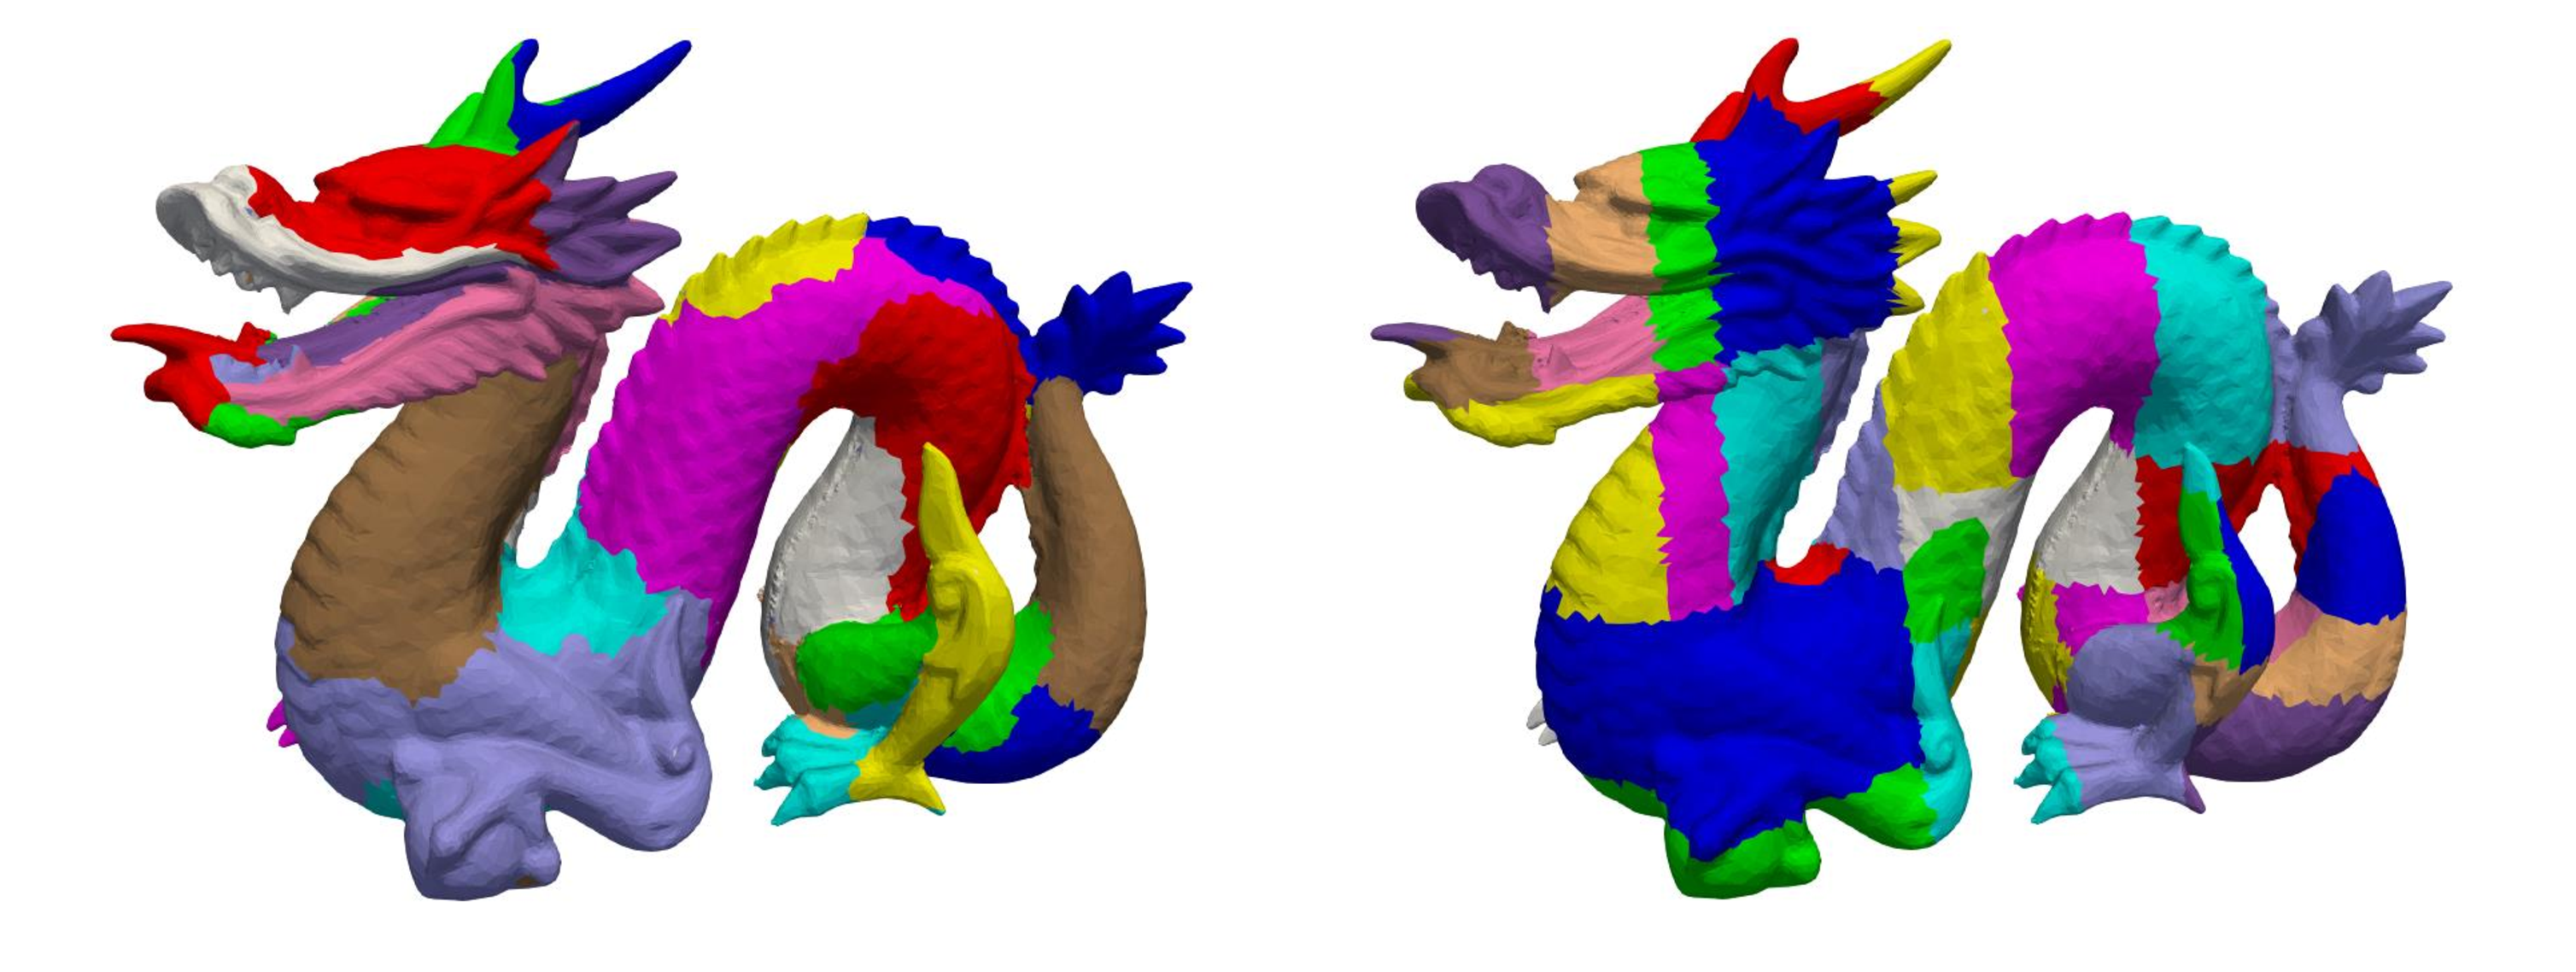
\includegraphics[width=1.0\textwidth]{./pics/text_2_smooth/decomp.pdf}
	\caption{Визуализация декомпозиции тестовой расчетной сетки dragon на 32 домена с помощью алгоритма Фархата (сверху) и иерархического алгоритма (снизу).}
	\label{fig:text_2_smooth_decomp}
\end{figure}

\begin{figure}[ht]
	\centering
	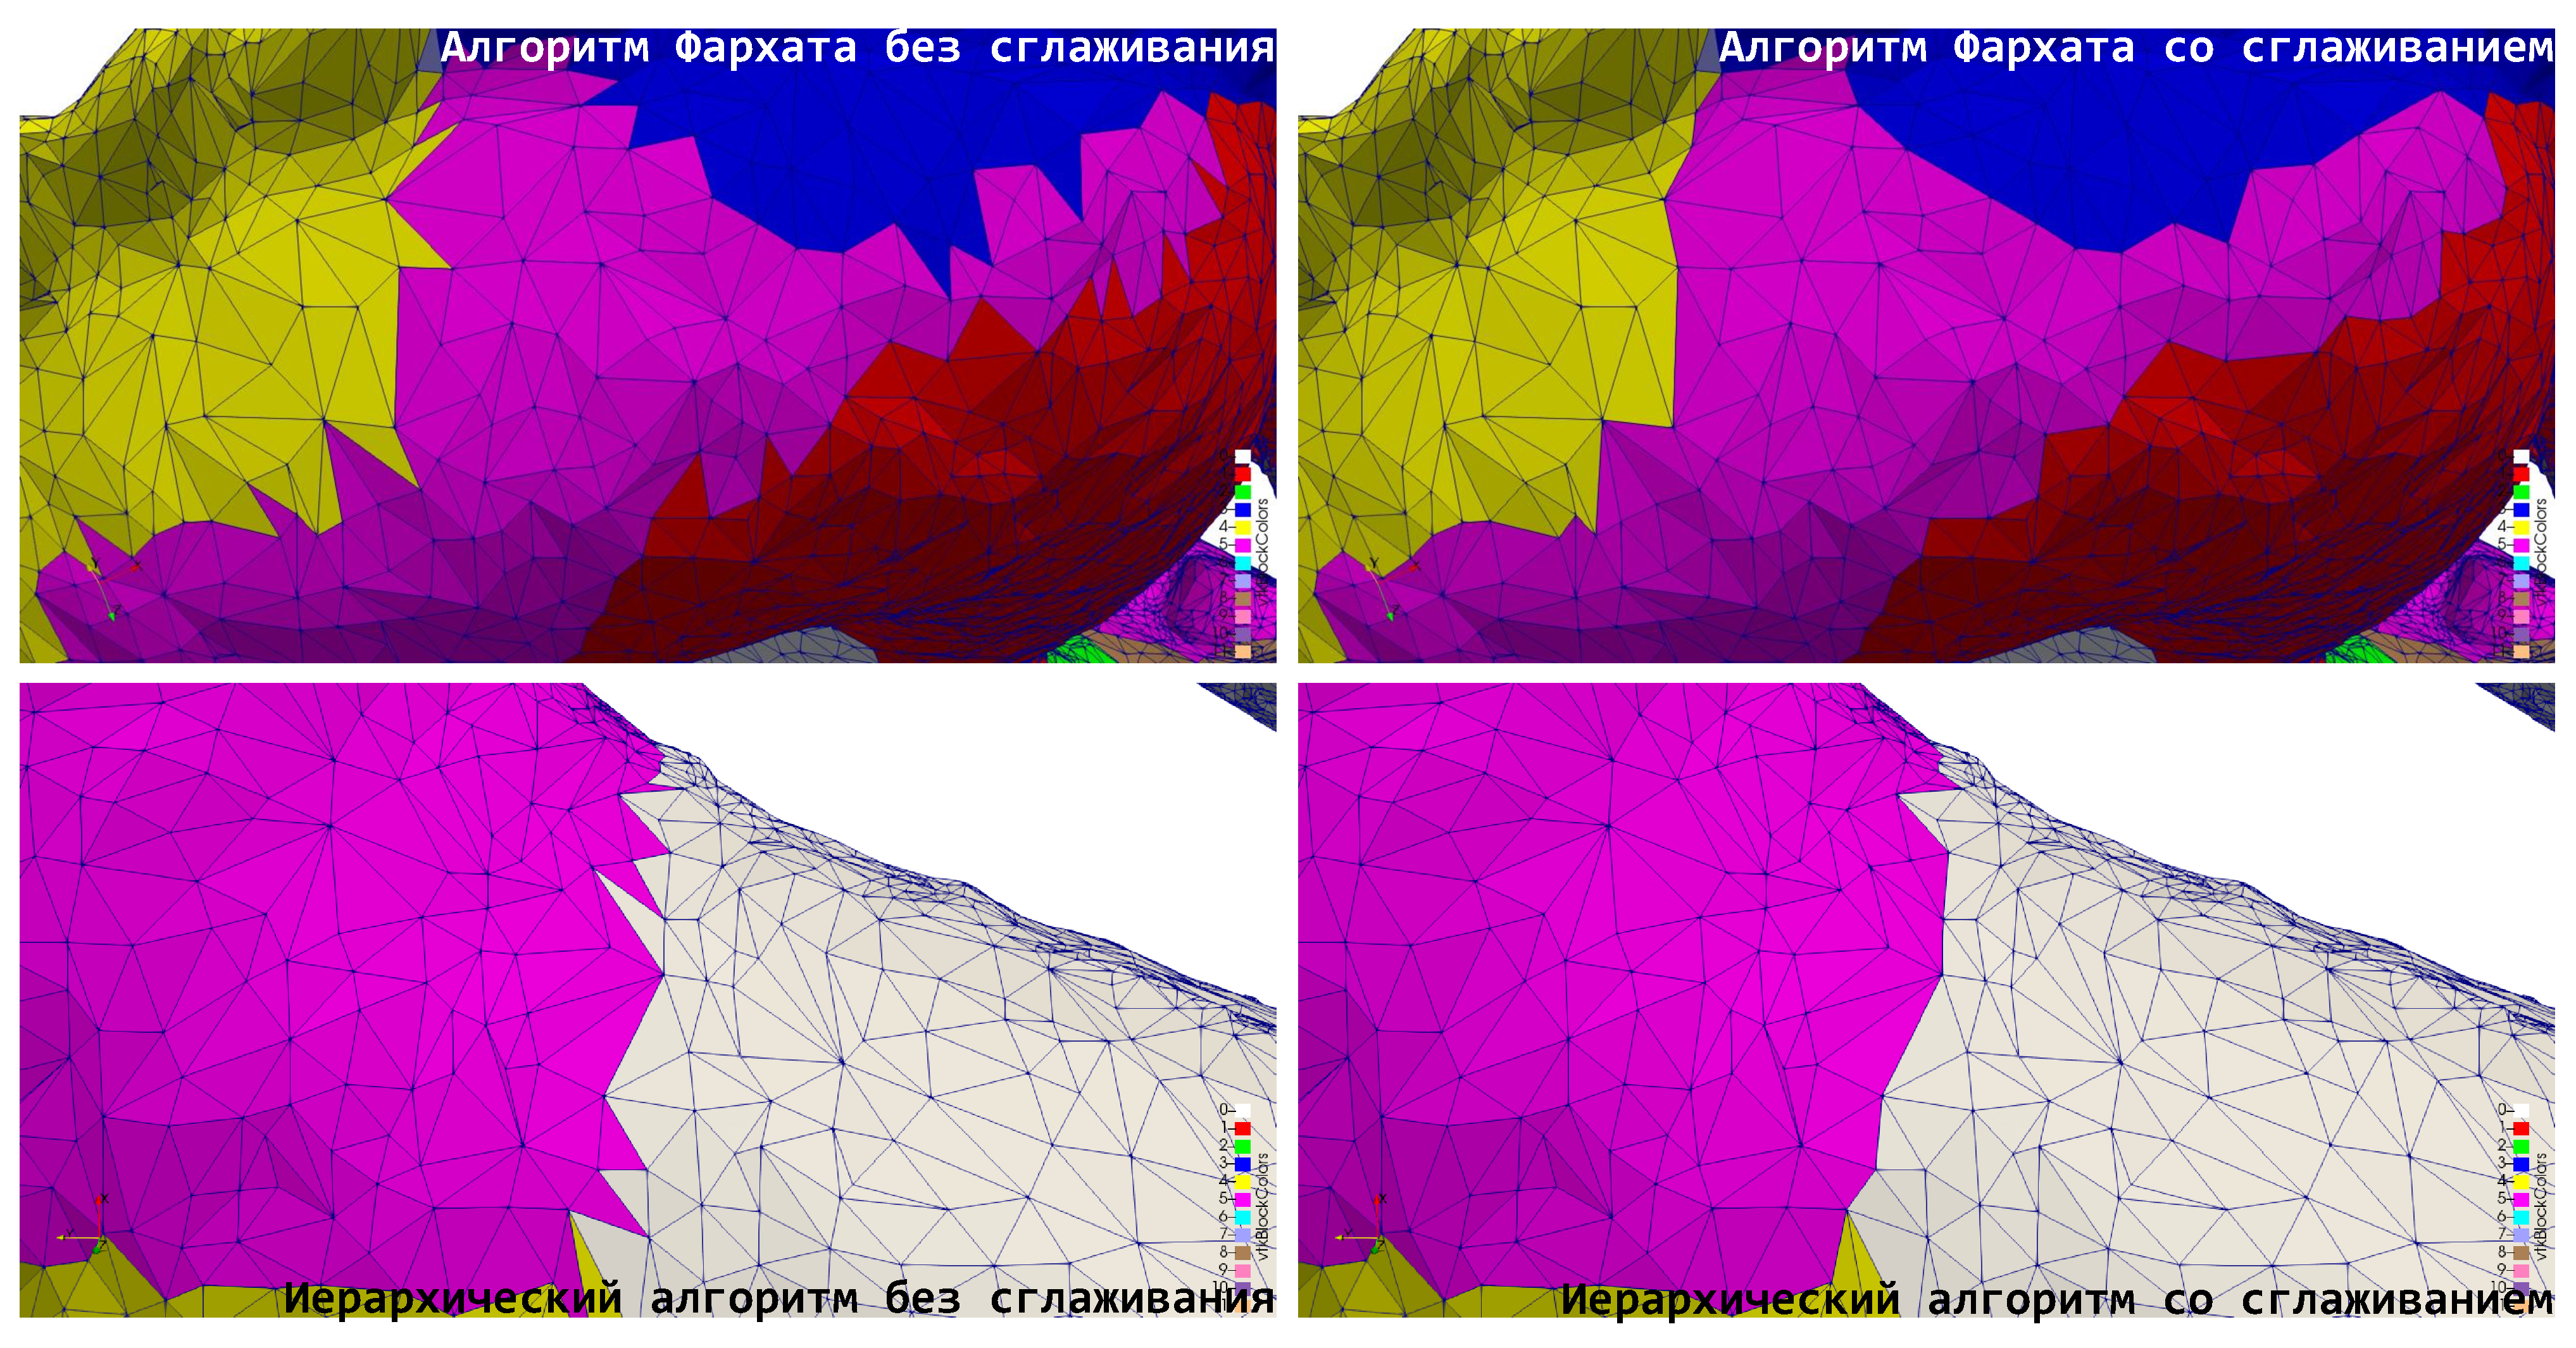
\includegraphics[width=0.8\textwidth]{./pics/text_2_smooth/decomp2.pdf}
	\caption{Визуализация применения сглаживания границ между доменами после работы алгоритма Фархата (сверху) и иерархического алгоритма (снизу).}
	\label{fig:text_2_smooth_decomp2}
\end{figure}

На рис.~\ref{fig:text_2_smooth_decomp} представлена визуализация декомпозиции тестовой расчетной сетки dragon с помощью алгоритма Фархата и иерархического алгоритма бинарной декомпозиции.
В обоих случаях декомпозиция выполнятся на 32 домена.
При этом на рис.~\ref{fig:text_2_smooth_decomp2} представлены результаты работы с уже примененным сглаживанием границ между доменами.

На рис.~\ref{fig:text_2_smooth_decomp2} крупным планом продемонстрированы отдельные части тестовой расчетной сетки dragon с отображением ребер ячеек.
На этом рисунке виден эффект от применения алгоритма сглаживания границ меду доменами, прежде всего от заключается в устранении одиноких ячеек, которые вторгаются в соседний домен одной своей вершиной.
После применения алгоритма границы между доменами визуально выглядят более гладко, их длина уменьшается.

\subsubsection{Результаты экспериментов}

Для тестирования эффективности алгоритма сглаживания границ между доменами использовались тестовые неструктурированные поверхностные сетки bunny, dragon, lucy, к которым были применены алгоритмы декомпозиции с показателем $D = 0$ и сравнены показатели качества декомпозиции до и после сглаживания границ.
Результаты проведения экспериментов представлены на рис.~\ref{fig:text_2_smooth_graphics}.

\begin{figure}[ht]
	\centering
		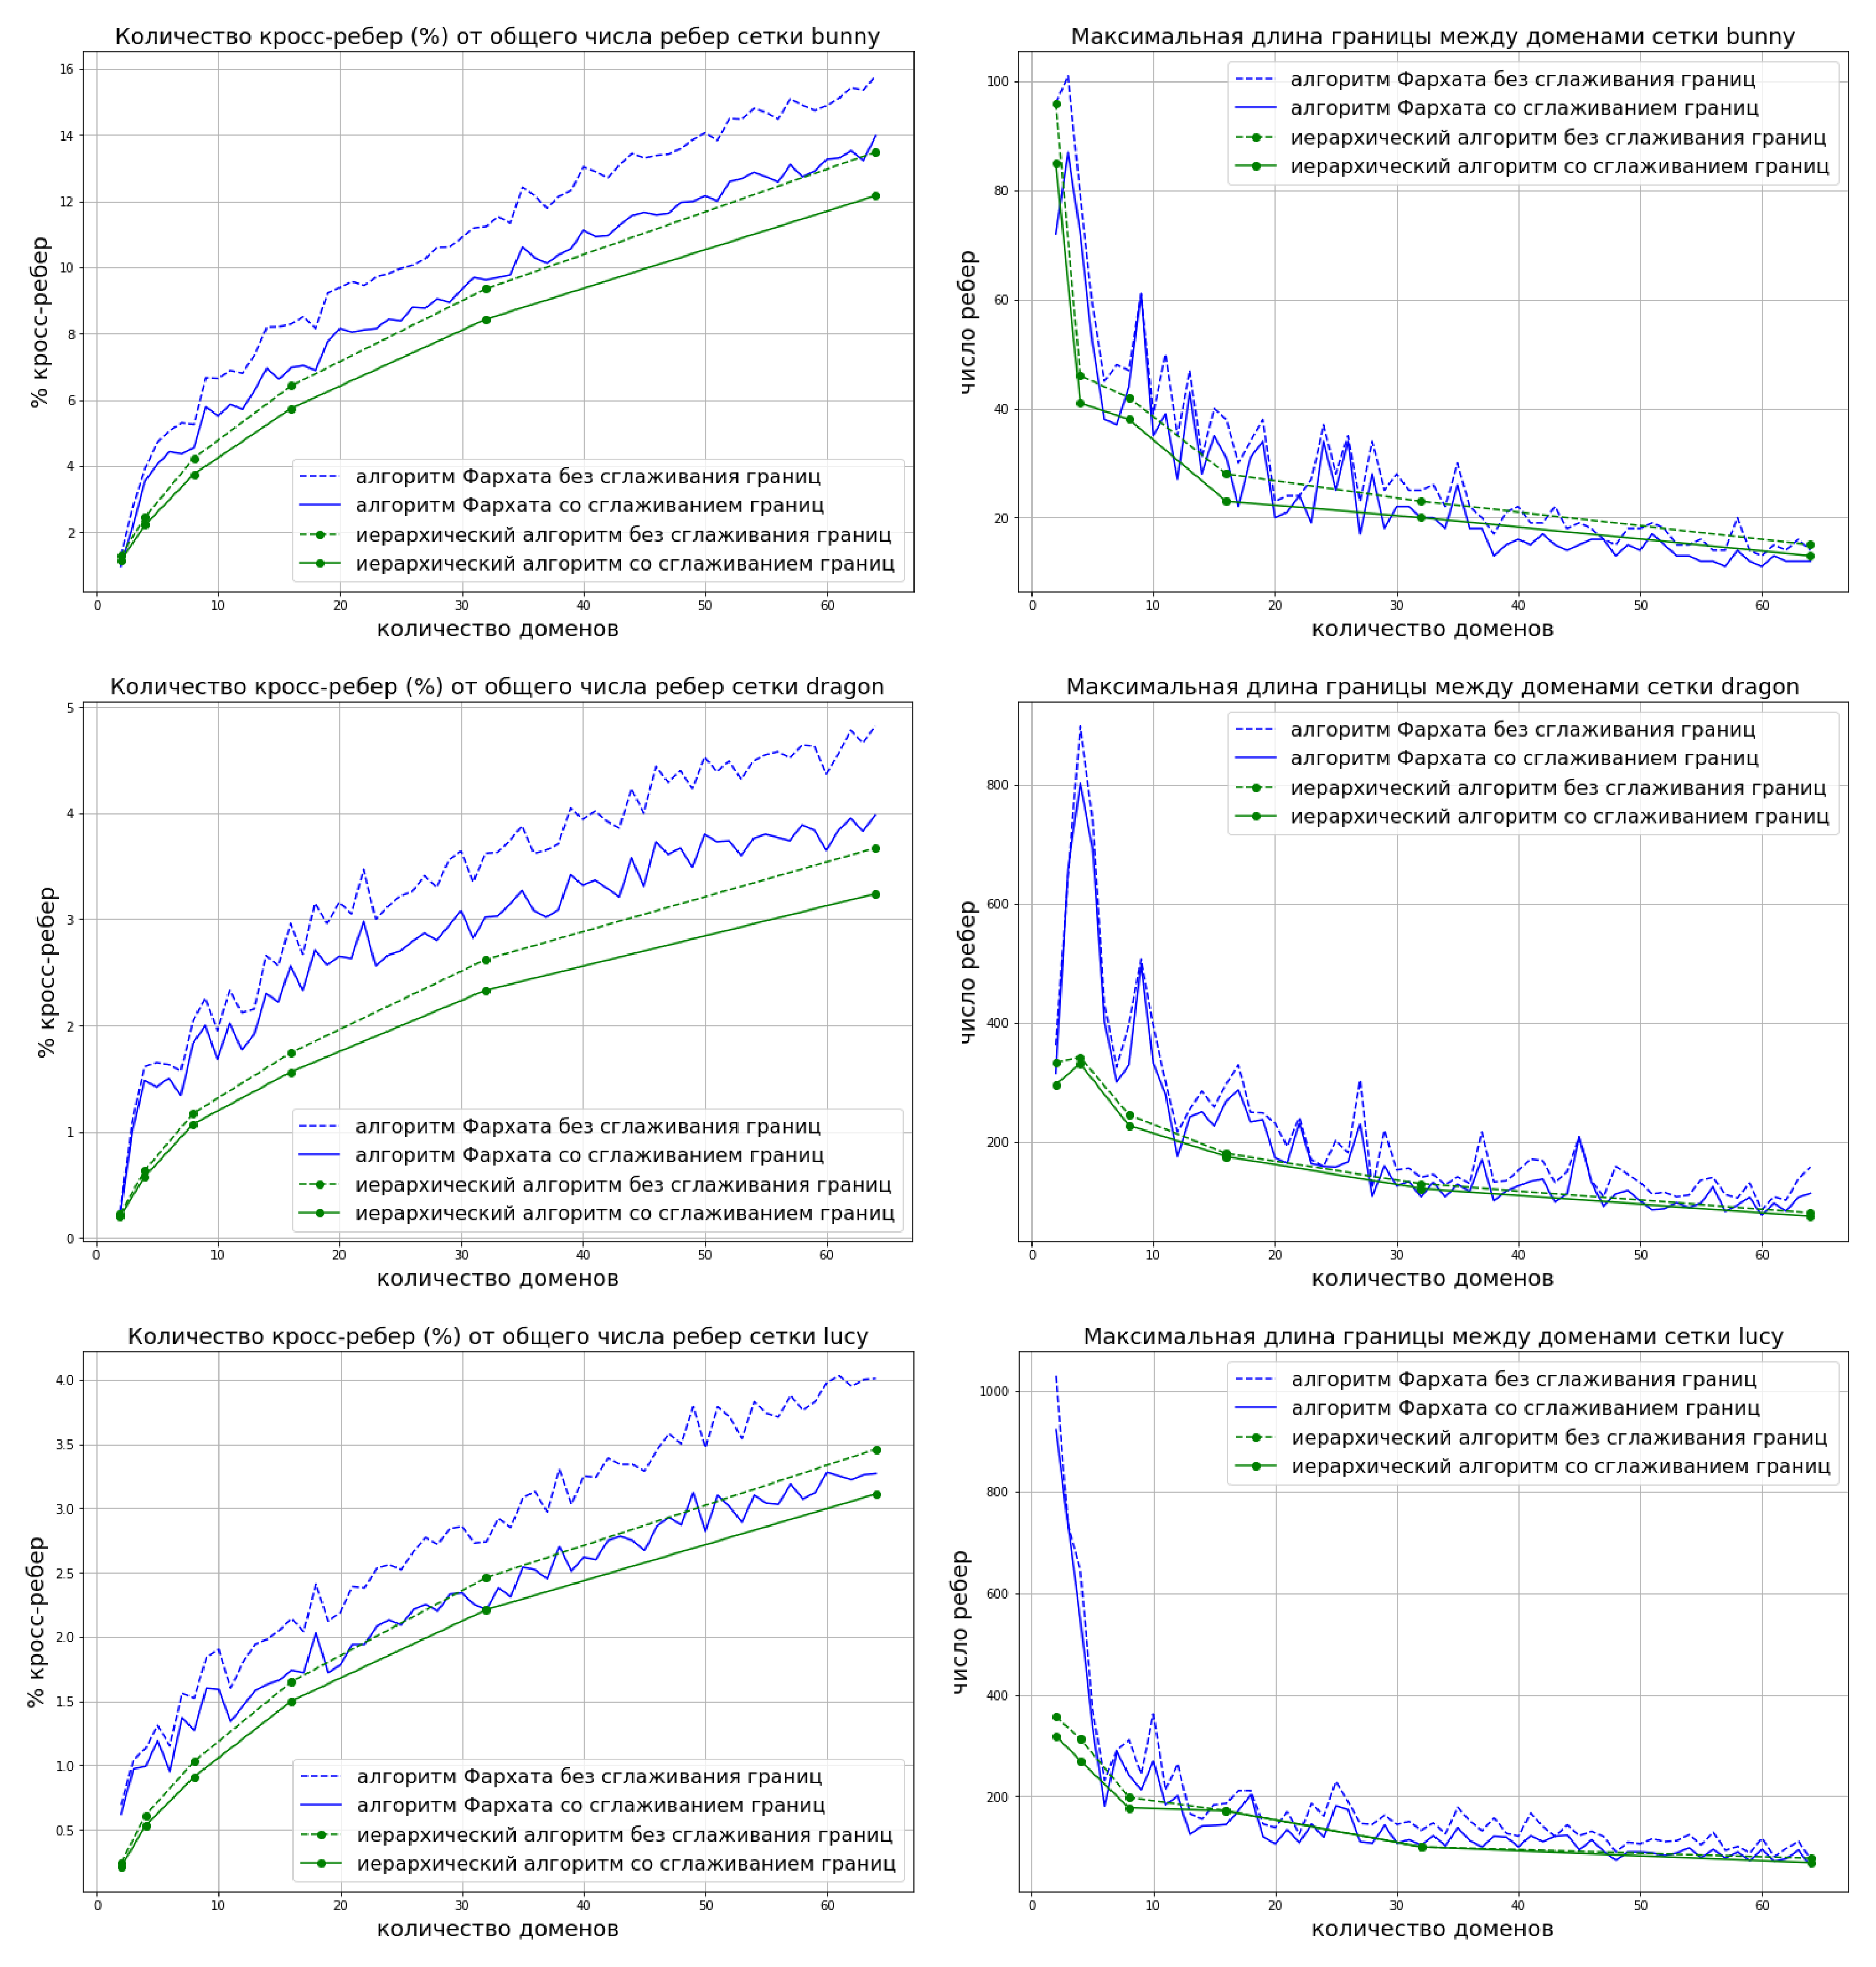
\includegraphics[width=0.8\textwidth]{./pics/text_2_smooth/graphics.pdf}
	\caption{Графики доли кросс-ребер (\%) от общего числа ребер сетки и максимальной длины границы между доменами при декомпозиции тестовых сеток bunny, dragon и lucy на количество доменов от 2 до 64.}
	\label{fig:text_2_smooth_graphics}
\end{figure}

Неструктурированные поверхностные расчетные сетки bunny (количество ячеек $5 \cdot 10^3$), dragon (количество ячеек $10^5$), lucy (количество ячеек $10^5$) были взяты из открытых источников.
Из приведенных на рис.\ref{fig:text_2_smooth_graphics} данных видно, что в целом проиллюстрированные показатели эффективности декомпозиции расчетных сеток (процентная доля ребер сетки, являющихся граничными ребрами между доменами, и максимальная длина границы между доменами) лучше для иерархического пространственного алгоритма декомпозиции.
Применение же алгоритма сглаживания границ приводит к сокращению как общего количества граничных ребер (кросс-ребер), так и длины максимальной границы примерно на 10\%.
Этот эффект приводит к снижению времени межпроцессных обменов для задач, выполняющих расчеты на поверхностных расчетных сетках.
